\chapter{Code Structure}
\section{Spatial discretization along homogeneous directions}
Our solver is based on a Fourier approach. Among the advantages of such approach we face the possibility to expansion of the unknown functions in terms of truncated Fourier series in the homogeneous directions. For example the wall-normal component $v$ of the velocity vector is represented as:
\begin{equation}
v(x,y,z,t) = \sum_{h=-nx/2}^{+nx/2} \sum_{l=-nz/2}^{+nz/2} \hat{v}_{hl}(y,t) e^{i\alpha x}e^{i \beta z}
\end{equation}
where:
\begin{equation}
\alpha = \frac{2\pi h}{L_{x}} = \alpha_{0} h; \quad \beta= \frac{2 \pi l}{L_{z}} = \beta_{0}l
\end{equation}

$h$ and $l$ are integer indexes corresponding to the streamwise and spanwise direction respectively, and $\alpha_{0}$ and $\beta_{0}$ are the fundamental wavenumbers in these directions, defined in terms of the streamwise and spanwise lengths $L_{x} = {2\pi}/{\alpha_{0}} $ and $L_{z} = {2 \pi}/{\beta_{0}}$ of the computational domain. The computational parameters given by the streamwise and spanwise lenght of the computational domain, $L_{x}$ and $L_{z}$ , and the truncation of the series, $nx$ and $nz$, must be chosen so as to miminize computational errors. For further details regarding the proper choice of a value of $L_{x}$ see~\cite{QuadrioMaurizio2003Issi}.

The convolutions required to solve the equations~\ref{curl:momentum:y} and~\ref{normal:velocity} are computationally expensive if carried out in the frequency domain. The same evaluation can be performed efficiently by first transforming the three Fourier components of velocity back in physical space, multiplying them in all six possible pair combinations and eventually retransforming the results into the Fourier space. Fast Fourier Transform algorithms are used to move from Fourier to physical space and viceversa. The aliasing error is removed by expanding the number of modes by a factor of at least $3/2$ before the inverse Fourier transforms, to avoid the introduction of spurious energy from the high-frequency into the low-frequency modes during the calculation~\cite{ns:quadrio}.





\section{Finite difference scheme}
The discretization of the wall-normal derivatives $D_{1}$, $D_{2}$ and $D_{4}$, required for the numerical solution of the present problem, is performed through finite difference (FD) compact schemes~\cite{finite:difference:scheme} with fourth-order accuracy over a computational molecule composed by five arbitrarily spaced grid points. We indicate here with $d_{1}^{j} (i), i = -2, \dots , 2$ the five coefficients discretizing the exact operator $D_{1}$ over five adjacent grid points centered at $y_{j}$ :
\begin{equation}
D_{1} \big( f(y) \big) \vert_{y=y_{j}} = \sum_{i=-2}^{2} d_{1}^{j} (i) f(y_{j+i})
\end{equation}
The basic idea of compact schemes can be most easily understood by thinking of a standard FD formula in Fourier space as a polynomial interpolation of a trascendent function, with the degree of the polynomial corresponding to the formal order of accuracy of the FD formula. Compact schemes improve the interpolation by replacing the polynomial with a ratio of two polynomials, i.e. with a rational function. This obviously increases the number of available coefficients, and moreover gives control over the behavior at infinity (in frequency space) of the interpolant, whereas a polynomial necessarily diverges. This allows a compact FD formula to approximate a differential operator in a wider frequency range, thus achieving resolution properties similar to those of spectral schemes~\cite{finite:difference:scheme}.
Compact schemes are also known as implicit finite-differences schemes, because they typically require the inversion of a linear system for the actual calculation of a derivative~\cite{compact:difference}\cite{finite:difference:scheme}.
 Here we are able to use compact, fourth-order accurate schemes at the cost of explicit schemes, owing to the absence of the third-derivative operator from the equations of motion. Thanks to this property, it is possible to find rational function approximations for the required three FD operators, where the denominator of the function is always the same, as highlighted first in the original Gauss-Jackson-Noumerov compact formulation exploited in his seminal work by Thomas~\cite{Thomas:coeff}, concerning the numerical solution of the Orr-Sommerfeld equations.\par
To illustrate Thomas’ method, let us consider an 4th-order one-dimensional ordinary differential equation, linear for simplicity, in the form:
\begin{equation}
D_{4}(a_{4}f) + D_{2}(a_{2}f)+D_{1}(a_{1}f)+a_{0}f = g,
\label{Thomas:coeff}
\end{equation}
Where the coefficients $a_{i}= a_{i}(y)$ are arbitrary functions of the independent variable $y$, and $g = g(y)$ is a known RHS. Let us moreover suppose that a differential operator, for example $D_{4}$, is approximated in frequency space as the ratio of two polynomials, say $\mathcal{D}_{4}$ and $\mathcal{D}_{0}$. Polynomials like $\mathcal{D}_{4}$ and $\mathcal{D}_{0}$ have their counterpart in physical space, and ${d}_{4}$ and $d_{0}$ are the corresponding FD operators. The key point is to impose that all the differential operators appearing in the example equation~\ref{Thomas:coeff} admit a representation such as the preceding one, in which the polynomial $\mathcal{D}_{0}$ at the denominator remains the same.\par
Equation~\ref{Thomas:coeff} can thus be recast in the new, discretized form:
\begin{equation}
d_{4} (a_{4}f) + d_{2} (a_{3}f) + d_{1} (a_{1}f) + d_{0} (a_{0}f) = d_{0} g,
\end{equation}
and this allows us to use explicit FD formulas, provided the operator $d_{0}$ is applied to the right-hand-side of our equations. The overhead related to the use of implicit finite difference schemes disappears, while the advantage of using high-accuracy compact schemes is retained~\cite{ns:quadrio}.





\subsection{Compute of the finite difference coefficients}










\section{Time Discretization}





\section{Domain Decompositions}
The engine of Quadrio and Luchini described into~\cite{cpl:presentazione} works per \emph{y-slabs}, as shown in figure~\ref{domain_decomp},
\begin{figure}
\centering
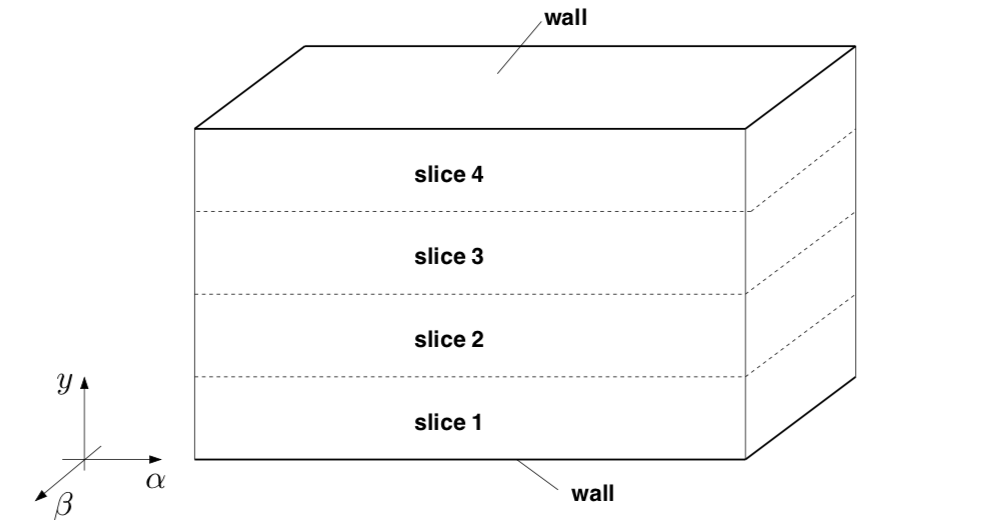
\includegraphics[width=0.8\textwidth]{grafici/decomp_dominio_cpl}
\caption{Original domain decomposition in case of 4 processors}
\label{domain_decomp}
\end{figure}
 allowing to perform convolutions and Fourier transformations locally on each processor, avoiding the cost of non-local transposition for the velocity array and the non-linear terms ones. Such implementation, denominated pipelined-linear-system (PLS), lead to a minimum of communication, in fact this approach require to send and receive only the values stored in the two upper and lower boundary cells of the local decomposition, in order to provide the data required by the fourth-order finite difference scheme.
 \par
 Using the PLS approach the number of bytes exchanged in a three step Range-Kutta method are:
 \begin{equation}
 D_{t} = 3 \times 8 \times (p-1) \frac{3}{2} \times \frac{nx}{p} \frac{nz}{p} \times ny \times 18
 \label{exchange:data:cpl}
 \end{equation}
 where:
 \begin{description}
  \item[3] takes into account the number of time steps;
  \item[8] for counting the bytes;
  \item[$\mathbf{(p-1)}$] is the number of nodes across which the exchange take place;
  \item[ $\mathbf{\frac{3}{2}}$ ] corresponds to the expansion in horizontal modes required by the dealiasing process;
  \item[ $\mathbf{\frac{nx}{p} \times \frac{nz}{p}}$] is the grid portion, for each plane, to exchange with the others nodes;
  \item[18] due to the 3 velocities plus the 6 products to be exchanged twice, before and after the FFT;
  \item[ny] takes into account the number of planes to be exchanged.
\end{description}
Further details about the PLS communications are available in \cite[\nopp chapter 4.2]{ns:quadrio}. \\
 \par
Although efficient for small processors grid, the performances of this approach falls quickly whether the processors number becomes comparable with \emph{ny}.  Furthermore the code structure limit the number of parallel process to be just a fraction of the \emph{ny} extension. \\
\par
To avoid such limitations and increase the number of parallel processes we decided to move from PLS approach to something different.
We have identified two possible solutions:
\begin{description}
  \item employ \textbf{slab} decomposition along x or z axis;
  \item employ \textbf{pencil} decomposition.
\end{description}
Both implementation require extensive use of the MPI paradigm and, possibly, a library to handle such decompositions.
\par
We opted to employ OpenMPI\cite{openmpi} for what concern the MPI paradigm, in particular we entrusted to the well established MPI standard 3.1\cite{MPI:standard}, using OpenMPI release 3.1.3.
The ideas behind the choice of such library rely on the fact the OpenMPI is released behind BSD license\cite{bsd:license}, it is designed to group different MPI implementation, avoiding fragmentation and forking problem\cite{faq:openmpi} and, although less optimized on proprietary fabric such as Intel Omni-Path fabric\cite{intel:omnipath}\cite{intel:intelmpivsopenmpi}, is likely the wider spreaded.
\par
For what concern the decomposition we entrusted in a new library, released by Steven Plimpton from the Sandia National Laboratories, called \emph{fftMPI}~\cite{fftMPI}. Such library leans on the MPI implementation, providing the proper cartesian communicator needed to perform the transposition of the arrays. Next to the communicator, this brand new library provide some useful tweak like permutations or the possibility to select the desired communication mode, which, compared with the FFTW-MPI Transpose\cite{FFTW05}\cite{FFTW:transpose} features, provide a wider personalization and reduce the work needed for the subsequent operations, such as the FFTs. 
\par
Finally is important to highlight that\emph{fftMPI} can handle both 1D and 2D decomposition, unlike FFTW-MPI.
Others similar libraries are P3DFFT\cite{p3dfft} from professor Dmitry Pekurovsky (UCSD), PFFT from professor Michael Pippig\cite{pfft} (Technische Universitat Chemnitz) and 2DECOMP\&FFT\cite{2decomp} by Ning Li.





\subsection{Slabs decomposition}
The concept of slab decomposition, or 1D decomposition, is quite simple. The domain is subdivided in slices, which turns out to be planes.


\subsection{Pencil decomposition}

